\documentclass[10.5pt,a4paper]{article}

\usepackage[a4paper,top=22mm,bottom=24mm,left=23mm,right=23mm,headheight=14pt]{geometry}
\usepackage[T1]{fontenc}
\usepackage[utf8]{inputenc}
\usepackage{lmodern}
\usepackage{microtype}
\usepackage{amsmath,amssymb}
\usepackage{booktabs,tabularx,longtable,array}
\usepackage{enumitem}
\usepackage{fancyhdr}
\usepackage{titlesec}
\usepackage{xcolor}
\usepackage{listings}
\usepackage{hyperref}
\usepackage{tikz}
\usetikzlibrary{arrows.meta,positioning,shapes.geometric}

\definecolor{ink}{HTML}{0A0A0A}
\definecolor{mid}{HTML}{555555}
\definecolor{rule}{HTML}{B8B8B8}
\hypersetup{
  colorlinks=true,
  linkcolor=ink,
  urlcolor=ink,
  citecolor=ink,
  pdftitle={KineGrant: Verifiable Authorization for Physical Actions},
  pdfauthor={Zoah},
  pdfsubject={KGP-001 Experimental Open Draft 0.1},
  pdfkeywords={physical AI, authorization, capabilities, action gate, receipts, robotics security}
}

\pagestyle{fancy}
\fancyhf{}
\fancyhead[L]{\footnotesize\sffamily\bfseries KINEGRANT}
\fancyhead[R]{\footnotesize\sffamily KGP-001 EXPERIMENTAL OPEN DRAFT 0.1}
\fancyfoot[L]{\footnotesize\sffamily 12 AUGUST 2026}
\fancyfoot[R]{\footnotesize\sffamily\thepage}
\renewcommand{\headrulewidth}{0.4pt}
\renewcommand{\footrulewidth}{0pt}

\titleformat{\section}{\Large\sffamily\bfseries}{\thesection}{0.8em}{}
\titleformat{\subsection}{\normalsize\sffamily\bfseries}{\thesubsection}{0.7em}{}
\titleformat{\subsubsection}{\normalsize\sffamily\bfseries}{\thesubsubsection}{0.6em}{}
\titlespacing*{\section}{0pt}{2.2em}{0.8em}
\titlespacing*{\subsection}{0pt}{1.6em}{0.5em}
\titlespacing*{\subsubsection}{0pt}{1.2em}{0.4em}

\setlength{\parindent}{0pt}
\setlength{\parskip}{0.58em}
\setlist{nosep,leftmargin=1.5em,topsep=0.35em}
\renewcommand{\arraystretch}{1.25}
\newcolumntype{Y}{>{\raggedright\arraybackslash}X}
\newcommand{\term}[1]{\textsf{\bfseries #1}}
\newcommand{\code}[1]{\texttt{#1}}
\newcommand{\statusline}[1]{\textsf{\footnotesize\bfseries #1}}
\newcommand{\note}[1]{\par\vspace{0.35em}\noindent\fbox{\parbox{0.94\linewidth}{\small #1}}\par\vspace{0.35em}}

\lstdefinestyle{kgp}{
  basicstyle=\ttfamily\footnotesize,
  backgroundcolor=\color{black!3},
  frame=single,
  rulecolor=\color{black!25},
  columns=fullflexible,
  keepspaces=true,
  breaklines=true,
  aboveskip=0.8em,
  belowskip=0.8em,
  xleftmargin=0.4em,
  xrightmargin=0.4em
}

\begin{document}

\thispagestyle{empty}
\vspace*{10mm}
{\sffamily\bfseries\large KINEGRANT PROTOCOL}\par
\vspace{25mm}
{\sffamily\bfseries\fontsize{32}{35}\selectfont KineGrant:\par
Verifiable Authorization\par
for Physical Actions}\par
\vspace{8mm}
{\sffamily\Large KGP-001 Experimental Open Draft 0.1}\par
\vspace{13mm}
{\large Zoah}\par
{\small 12 August 2026}\par
\vfill
\begin{tabularx}{\linewidth}{@{}Y Y Y@{}}
\toprule
\statusline{PROTOCOL} & \statusline{IMPLEMENTATION} & \statusline{LICENSE} \\
KGP-001 Draft 0.1 & Reference v0.1.1 & Apache-2.0 \\
\bottomrule
\end{tabularx}
\vspace{7mm}
{\footnotesize\color{mid}\begin{minipage}{\linewidth}
Independent experimental open project. This document does not claim standardization,
certification, production readiness, legal authority, or functional-safety compliance.
\end{minipage}}
\newpage

\begin{abstract}
Machines controlled by software increasingly cause state changes in the physical world.
The software that decides what to do is often separated from the device that ultimately
acts, while identity systems, transport security, robot middleware, and safety controls
each protect a different boundary. This leaves a narrow but important question: what
cryptographically verifiable authorization did this actuator possess for this exact
action, at this target, at this time?

KineGrant is an experimental authorization and accountability protocol for that boundary.
It converts a policy decision into a short-lived, signed, request-bound capability; places
a fail-closed action gate in the actuator control path; consumes the capability atomically;
and binds execution to a signed terminal receipt. The protocol is transport-independent,
defaults to denial, applies deny-overrides, and prevents untrusted policy sources from
expanding authority. This paper defines the system and threat models, decision semantics,
capability construction, gate algorithm, receipt semantics, conditional security
invariants, interoperability boundaries, and a reproducible software test method.

KineGrant does not solve identity enrollment, legal ownership, safe motion, sensor truth,
key compromise, or actuator firmware compromise. A receipt proves an executor's signed
attestation, not physical truth. The draft is intended to make the authorization boundary
precise enough to implement, attack, reproduce, and revise.
\end{abstract}

\tableofcontents
\newpage

\section{Introduction}

An AI system may infer an action, a robot application may transmit it, and a device may be
technically capable of carrying it out. None of those facts establishes that the action was
authorized. Intelligence is not permission.

Existing mechanisms provide essential controls: identity and access management authenticates
principals; public-key infrastructure authenticates keys and endpoints; network controls limit
connectivity; robot middleware governs communications; industrial protocols secure sessions;
and functional-safety systems constrain hazardous behavior. These controls should remain in
place\cite{ros2,opcua,matter}. The missing object addressed here is narrower: a device-verifiable grant that binds a
specific request to a policy evaluation and can be consumed immediately before a physical
action, followed by a signed result record.

KineGrant defines the following path. Its use of the term capability follows the security
tradition of unforgeable authority-bearing references, while adding protocol-specific request,
time, replay, and receipt semantics\cite{dennis,miller}.

\begin{center}
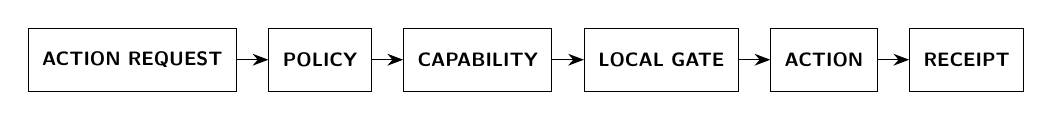
\begin{tikzpicture}[
  node distance=4mm,
  n/.style={draw=black,minimum height=8mm,inner xsep=5pt,font=\sffamily\scriptsize\bfseries},
  a/.style={-{Stealth[length=2mm]},line width=0.5pt}
]
\node[n] (r) {ACTION REQUEST};
\node[n,right=of r] (p) {POLICY};
\node[n,right=of p] (c) {CAPABILITY};
\node[n,right=of c] (g) {LOCAL GATE};
\node[n,right=of g] (a1) {ACTION};
\node[n,right=of a1] (x) {RECEIPT};
\draw[a] (r)--(p); \draw[a] (p)--(c); \draw[a] (c)--(g);
\draw[a] (g)--(a1); \draw[a] (a1)--(x);
\end{tikzpicture}
\end{center}

The protocol contributes four coupled properties. First, authorization is explicit and bound
to normalized request and policy digests. Second, permission is short-lived and single-use by
default. Third, the gate is placed in the trusted path to the actuator and fails closed. Fourth,
the outcome is represented by a signed, privacy-minimized terminal receipt.

The construction is not a claim that cryptography alone controls the physical world. Its
security properties are conditional on trusted keys, time, policy provenance, canonical
encoding, durable atomic replay state, and an actuator path that cannot bypass the gate. These
conditions are part of the protocol's deployment contract, not implementation details to be
assumed away.

\section{Scope and Design Goals}

\subsection{Goals}

KGP-001 is designed to provide:

\begin{enumerate}
  \item \textbf{Exact binding.} A grant identifies one agent, target, action, purpose,
  request digest, and policy snapshot digest.
  \item \textbf{Local verification.} A gate can decide without consulting a remote ledger
  or policy service at action time.
  \item \textbf{Bounded authority.} A capability is short-lived, scoped, and consumed once
  by default.
  \item \textbf{Monotonic restriction.} Untrusted policy and discovery inputs may restrict
  or deny but cannot create new permission.
  \item \textbf{Accountability.} Execution produces a signed terminal attestation that can
  be checked independently against explicit trust anchors.
  \item \textbf{Interoperability.} The authorization object can complement existing identity,
  middleware, device, and safety systems without replacing them.
\end{enumerate}

\subsection{Non-goals}

KineGrant is not a robot operating system, motion planner, functional-safety controller,
identity registry, legal authorization system, blockchain, token, or consensus network. It
does not establish ownership, infer human intent, determine whether sensor data is true, or
prove that a physical event occurred exactly as reported. It does not permit a software grant
to override a native safety veto or emergency stop.

\note{A conforming deployment evaluates physical execution as a conjunction: native platform
authorization AND a valid KineGrant capability AND the local safety controller must all allow.
Any layer may veto. KineGrant cannot force another layer to permit.}

\section{System and Threat Models}

\subsection{Entities and trust boundaries}

\begin{tabularx}{\linewidth}{@{}p{31mm}Y@{}}
\toprule
\textbf{Entity} & \textbf{Role and trust condition} \\
\midrule
Agent & Requests an action. It may be buggy or compromised; its request is not permission. \\
Policy source & Supplies rules. An allow rule is effective only if its issuer is independently
authenticated and explicitly trusted. \\
Policy engine & Evaluates normalized rules using trusted local time and produces a decision. \\
Authority & Signs capabilities. Its key and issuer identity are explicit gate trust anchors. \\
Action gate & Verifies, binds, and atomically consumes a capability in the actuator control path. \\
Replay store & Implements durable, linearizable consume-if-absent semantics for capability nonces. \\
Executor & Performs or supervises the action and signs one terminal receipt. \\
Verifier & Checks signatures, hashes, time, chain structure, and caller-supplied trust anchors. \\
Safety controller & Independently enforces motion, collision, process, and emergency constraints. \\
\bottomrule
\end{tabularx}

\subsection{Adversary capabilities}

The draft considers an adversary that can observe, delay, replay, reorder, and modify network
messages; submit stale or future-dated requests; inject policy documents; exploit ambiguous
adapters; attempt to substitute a target or action; race concurrent gate calls; restart a
process; and tamper with an unanchored receipt log. A robot application may be compromised and
may request or attempt a different action after receiving a capability.

The draft does not defeat theft of a trusted authority or executor key, compromised actuator
firmware that bypasses the gate, a dishonest executor or sensor, denial of service, traffic
analysis, physical coercion, or disputed legal authority. These remain explicit residual risks.

\subsection{Assumptions}

The arguments in Section~\ref{sec:analysis} require: (A1) Ed25519 signatures are unforgeable for
uncompromised keys; (A2) SHA-256 is collision resistant for the bound objects; (A3) the gate has
an authenticated trusted-issuer set; (A4) policy trust is established outside policy content;
(A5) gate time is sufficiently trustworthy; (A6) nonce consumption is durable and atomic; and
(A7) every protected actuator command traverses the conforming gate. Violating an assumption
invalidates the associated claim.

\section{Protocol Objects}

Let $H(x)$ be SHA-256 over the protocol's deterministic encoding of normalized object $x$.
Let $\operatorname{Sig}_{sk}(x)$ denote an Ed25519 signature and
$\operatorname{Verify}_{pk}(x,\sigma)$ its verification\cite{rfc8032}. Draft 0.1 uses deterministic JSON;
a later draft should adopt a standards-track canonical encoding such as JCS or deterministic
CBOR\cite{rfc8785}. Cross-implementation digest agreement is therefore a conformance requirement and an
identified migration item.

\subsection{Action request}

An action request is the tuple
\[
  r=(rid,agent,target,action,purpose,t_{issued},context).
\]
The request identifier is globally unique. Identifiers and action names are normalized before
evaluation. The request's timestamp is evidence supplied by the requester; it is not the clock
used to decide policy validity. The policy engine rejects requests older than the configured
maximum age or unreasonably far in the future according to trusted local time.

\subsection{Policy rule and normalized snapshot}

A rule contains an identifier, issuer, effect in $\{allow,deny\}$, target pattern, subjects,
actions, purposes, constraints, obligations, and optional validity window. The engine defaults
to denial and applies deny-overrides. Unknown authorization fields, constraints, or operators
fail closed. Missing target, subject, action, or purpose scope cannot be silently expanded into
a wildcard.

For a request $r$, time $t$, rule set $P$, and independently configured trusted allow-issuer
set $T_P$, define $Applicable(p,r,t)$ only when every normalized selector and every understood
constraint matches. Define:
\begin{align*}
D(r,P,t) &\equiv \exists p\in P:\ p.effect=deny \land Applicable(p,r,t),\\
A(r,P,T_P,t) &\equiv \exists p\in P:\ p.effect=allow \land p.issuer\in T_P
                 \land Applicable(p,r,t).
\end{align*}
The decision function is
\[
Outcome(r,P,T_P,t)=
\begin{cases}
deny & \text{if request freshness is invalid, parsing is incomplete, or }D(r,P,t),\\
allow & \text{if }A(r,P,T_P,t),\\
deny & \text{otherwise.}
\end{cases}
\]
This construction makes restriction monotonic with respect to untrusted sources: adding an
untrusted document cannot turn a denial into an allowance.

The decision records $H(r)$, outcome, reason, matched policy identifiers, obligations, and
$H(N(P,T_P))$, where $N$ is the complete normalized policy snapshot together with the trusted
issuer set used for evaluation. Binding the full snapshot prevents a policy-content change from
retaining the same digest merely because a small subset of identifiers is unchanged.

\subsection{Physical action capability}

Only an allowed decision may produce a capability. Its signed body contains at least:
\[
C=(v,cid,issuer,agent,target,action,purpose,H(r),H(N(P,T_P)),n,t_{nb},t_{exp}).
\]
Here $n$ is a cryptographically random nonce, $t_{nb}$ is not-before time, and $t_{exp}$ is the
exclusive expiry. The interval is half-open: $[t_{nb},t_{exp})$. KGP-001 limits capability
lifetime to 300 seconds and requires single-use consumption by default. Unknown versions,
unknown fields, malformed base64url, or invalid time ordering are rejected.

\subsection{Physical action receipt}

A terminal receipt contains the executor identity, capability identifier, request digest,
result, execution time interval, optional evidence hash, optional previous-receipt hash, and
executor signature. The receipt is constructed from the gate's verified capability result, not
from caller-reconstructed fields. A receipt log rejects a second terminal receipt for the same
capability. Raw video, audio, precise location, or personal data should remain outside the
receipt and may be referenced by a content hash when policy permits.

\section{Authorization and Execution Protocol}

\subsection{Issuance}

The policy engine evaluates request $r$ against normalized rules and trusted local time. If the
result is denial, no capability is issued. If allowed, the authority constructs $C$, chooses a
fresh nonce, applies a lifetime no longer than 300 seconds, and signs the deterministic encoding.
The authority does not make the decision self-authenticating: the gate separately authenticates
the capability issuer against its own trust configuration.

\subsection{Gate algorithm}

The following abstract algorithm is normative in ordering where the order affects authority.
An implementation may reject earlier for resource protection, but it must never invoke the
actuator before all checks and successful atomic consumption.

\begin{lstlisting}[style=kgp]
AUTHORIZE_AND_CONSUME(signed_capability, observed_request, trusted_now):
  body, signature := STRICT_PARSE(signed_capability)
  require body.version == "0.1"
  require NO_UNKNOWN_FIELDS(body)
  require body.issuer in TRUSTED_CAPABILITY_ISSUERS
  require VERIFY_ED25519(body.issuer_key, body, signature)
  require body.not_before < body.expires_at
  require body.expires_at - body.not_before <= 300 seconds
  require body.not_before <= trusted_now < body.expires_at
  require body.request_digest == H(NORMALIZE(observed_request))
  require EXACT_MATCH(body, observed_request,
                      [agent, target, action, purpose])
  require VALID_POLICY_DIGEST(body.policy_digest)
  require ATOMIC_CONSUME_IF_ABSENT(body.nonce) == CONSUMED
  return VERIFIED_CAPABILITY(body)
\end{lstlisting}

If any requirement fails, the gate returns denial and does not call the protected actuator.
The atomic operation must be linearizable for concurrent attempts and durable across the restart
boundary claimed by the deployment. A memory-only replay store is appropriate for simulation,
not a durable real device.

\subsection{Execution and receipt}

The executor receives the opaque verified result from the gate, performs the independently safe
action if all native controls also allow, and signs one terminal receipt. The receipt result may
record success, denial, failure, or interruption according to the protocol profile. Receipt
verification checks deterministic encoding, signature, caller-controlled executor trust,
capability binding, time consistency, evidence-hash syntax, previous hash, and terminal
uniqueness.

\section{Security Invariants and Analysis}\label{sec:analysis}

The following are conditional protocol arguments, not a machine-checked proof, certification,
or claim of immunity from implementation defects.

\subsection{I1: no grant, no protected action}

Under A3, A5, and A7, a protected actuator invocation can follow only a successful gate result.
The gate returns success only after issuer, signature, lifetime, request binding, and replay
checks. Therefore an absent, malformed, untrusted, expired, mismatched, or replayed capability
cannot authorize the protected invocation. This invariant does not hold if another firmware or
control path can reach the actuator without the gate.

\subsection{I2: request non-substitutability}

Under A1 and A2, changing agent, target, action, purpose, or any normalized request field changes
$H(r)$ or the exact bound field. The adversary must then either forge the authority signature,
find a digest collision, or cause divergent normalization. Strict schemas and conformance vectors
reduce, but do not eliminate, the normalization risk.

\subsection{I3: at-most-once authorization}

Under A6, all successful uses of nonce $n$ linearize at the consume-if-absent operation. At most
one transition from absent to consumed exists. Consequently, concurrent, later, and post-restart
replays are denied. This is an authorization property: an actuator or network fault could still
make the physical result ambiguous, so idempotence and safe recovery remain device concerns.

\subsection{I4: bounded validity}

Under A5, the half-open interval check accepts $C$ only when
$t_{nb}\leq t<t_{exp}$ and $t_{exp}-t_{nb}\leq300$ seconds. The exact instant
$t=t_{exp}$ is denied. Requester-controlled timestamps cannot revive policy because policy
windows and freshness are evaluated against the engine's trusted time.

\subsection{I5: receipt integrity, not physical truth}

Under A1 for an explicitly trusted executor, alteration of a signed receipt or its referenced
hashes is detectable. A previous-receipt hash makes deletion or reordering detectable after a
later trusted checkpoint is retained. Neither property establishes that the executor or sensor
reported reality honestly. Independent attestation and observation are separate systems.

\subsection{Attack analysis}

\begin{longtable}{@{}p{34mm}p{57mm}p{62mm}@{}}
\toprule
\textbf{Attempt} & \textbf{Required response} & \textbf{Residual condition} \\
\midrule
\endhead
Forged capability & Reject invalid signature or untrusted issuer. & Trusted authority key theft
is outside the software-only model. \\
Request mutation & Reject digest or exact field mismatch. & Divergent normalization across
implementations must be tested. \\
Replay & Reject already-consumed nonce atomically. & Store must be durable and linearizable for
the deployment boundary. \\
Concurrent replay & Exactly one consume operation may succeed. & Distributed stores require a
documented consistency model. \\
Expired capability & Reject when $now\geq expires\_at$. & Clock rollback or compromise remains a
deployment threat. \\
Policy injection & Untrusted issuer cannot produce allow; applicable deny may restrict. & Trust
configuration compromise remains possible. \\
Backdated request & Evaluate policy time against trusted now; apply request-age limits. & Secure
time synchronization remains necessary. \\
Ambiguous adapter & Reject unknown field, constraint, operator, or prohibition. & A known but
incorrect mapping remains an adapter defect. \\
Receipt substitution & Verify expected capability, request digest, executor trust, and signature.
& A trusted executor can still lie about physical reality. \\
Gate bypass & Deployment is non-conforming. & Requires hardware and control-path architecture,
not a message-format fix. \\
Safety conflict & Native safety veto remains authoritative. & KineGrant is not a safety case. \\
\bottomrule
\end{longtable}

\section{Interoperability Boundaries}

KineGrant complements existing systems by adding action-specific, short-lived authority at the
local actuation boundary. It should reuse existing identities, keys, transports, and native
authorization rather than duplicate them.

\begin{tabularx}{\linewidth}{@{}p{28mm}p{52mm}Y@{}}
\toprule
\textbf{System} & \textbf{What it already provides} & \textbf{KineGrant boundary} \\
\midrule
IAM / PKI & Principal and key identity, authentication, trust distribution. & Supplies trust
anchors; KineGrant binds them to one physical action and time window. \\
ROS 2 / SROS2 & Enclave identity and middleware communication permissions. & A bridge gates the
specific actuator command; middleware permission remains required. \\
OPC UA & Secure channels, application/user identity, roles, audit mechanisms. & A method adapter
binds a capability to an exact node/method/action without weakening OPC UA controls. \\
Matter & Authenticated fabrics, device interaction, and message replay protection. & A target
adapter adds protocol-level action authorization; Matter authorization remains authoritative. \\
W3C ODRL & Policy vocabulary for permissions, prohibitions, duties, and constraints. & A strict
profile normalizes understood constructs and rejects unknown authorization semantics. \\
W3C WoT TD & Machine-readable affordances, forms, and security metadata. & Discovery may publish
identity and policy pointers; unauthenticated discovery cannot grant. \\
Functional safety & Hazard controls, safe state, emergency handling, motion limits. & Always
independent and veto-capable; never replaced by a capability. \\
\bottomrule
\end{tabularx}

The mappings use published platform and policy models as reference points, including ODRL and
WoT Thing Description\cite{odrl,wot}. Adapters are security boundaries. They must record source profile and transport, safely encode
target components, reject caller attempts to overwrite system-owned context, and fail closed on
unknown authorization constructs. Draft 0.1 does not claim conformance certification with the
systems listed above.

\section{Receipts, Privacy, and Auditability}

An audit record is useful only if its claim is stated precisely. A KineGrant receipt supports the
claim: ``the holder of this executor key signed this terminal statement about the identified
capability and request.'' With an explicit trusted-executor set, the verifier may additionally
claim that the signer was trusted for the verification context. The receipt alone cannot support
the stronger claim that a sensor was accurate or that a physical event occurred.

Privacy minimization is therefore structural. The base receipt carries identifiers, time,
result, digests, and signatures. Rich evidence stays out of band. A hash can commit to external
evidence, but collection, retention, disclosure, and deletion require independent policy and law.
Receipt chains should be checkpointed outside the executor to make later deletion detectable;
no public or consortium ledger is required in the real-time safety path.

\section{Reference Implementation and Reproducible Evidence}

The Apache-2.0 Python reference implementation is version 0.1.1; the wire protocol remains draft
0.1. It demonstrates Ed25519 capability and receipt signatures, default-deny policy evaluation,
trusted policy and capability issuers, deterministic JSON digests, strict data models and JSON
Schemas, in-memory and SQLite replay stores, adapters, a gate, and receipt verification.

Release v0.1.1 was validated with 33 automated protocol and security regression tests across the
documented environment, a demo smoke test, Draft 2020-12 JSON Schema validation, and wheel/source
package builds\cite{jsonschema}. The separate Machine Permission Test (MPT) v0.1 publishes nine machine-readable
cases:

\begin{enumerate}
  \item no capability: deny;
  \item valid capability: exactly one authorization;
  \item replay: deny;
  \item mutation of agent, target, action, or purpose: deny;
  \item wrong capability issuer: deny;
  \item expired capability: deny;
  \item concurrent use: exactly one success;
  \item restart followed by replay: deny;
  \item receipt tampering or untrusted executor: deny.
\end{enumerate}

The reference evidence reports 9/9 PASS. This is project-generated software evidence, not an
independent audit, formal proof, physical-device validation, or safety certification. A useful
external reproduction must record exact repository commit, runtime, operating system,
dependencies, command, raw evidence, and cryptographic hashes; failures and deviations should be
published rather than summarized away.

\begin{lstlisting}[style=kgp]
git clone https://github.com/zoahdev/kinegrant-protocol.git
cd kinegrant-protocol
python -m venv .venv
# activate the environment, then:
python -m pip install -e '.[test]'
kinegrant-mpt --output machine-permission-test.evidence.json
python -m unittest discover -s tests -v
\end{lstlisting}

The authoritative commands, checksums, release assets, and platform-specific instructions are
maintained in the repository and release notes. Reproduction establishes behavior in the tested
software environment only.

\section{Deployment Requirements}

A real deployment claiming KGP-001 behavior should document and review at least the following:

\begin{enumerate}
  \item place the gate in the mandatory actuator control path;
  \item keep native authorization and an independent functional-safety controller enabled;
  \item store authority and executor keys in hardware-backed keystores where available;
  \item provision issuer trust and revocation independently of untrusted input;
  \item use monotonic or securely synchronized time and define clock-failure behavior;
  \item provide durable, atomic nonce consumption across the stated restart and concurrency scope;
  \item pin adapter profiles and reject unknown or ambiguous constructs;
  \item minimize receipt data and checkpoint receipt-chain state outside the executor;
  \item fail safe when policy, adapter, registry, time, or replay services are unavailable;
  \item complete independent cryptographic, software, privacy, and machinery-safety review.
\end{enumerate}

The protocol should not be the sole control for hazardous machinery. A deployment report should
identify bypass paths, trusted computing base, key lifecycle, update mechanism, storage failure
modes, time source, action recovery semantics, and test evidence.

\section{Open Problems}

Draft 0.1 intentionally leaves several issues unresolved: conflicts among legitimate co-owners;
revocation during a running action; delegation and attenuation; multi-agent actions; privacy-
preserving discovery; emergency and accessibility override semantics; hardware-backed actuator
attestation; distributed replay-store consistency; cross-language canonicalization; long-running
actions whose duration exceeds grant lifetime; and formal verification of policy adapters and
gate implementations.

These are not roadmap decorations. Each affects the meaning of authorization and should be
resolved through explicit threat models, test vectors, incompatible-change rules, and public
review before a stable protocol claim.

\section{Conclusion}

Physical AI creates a boundary where an intention represented in software becomes an action in
the world. KineGrant isolates one question at that boundary: did this actuator receive a valid,
specific, short-lived, non-replayable authorization for this request, and can the executor's
terminal statement be verified later?

KGP-001 answers with a policy decision, signed capability, mandatory local gate, atomic
consumption, and signed receipt. Its value depends less on the novelty of any cryptographic
primitive than on composing the trust boundaries without silently widening authority. The draft
therefore favors explicit trust, exact binding, default denial, short lifetimes, local verification,
and falsifiable evidence. Its current status remains an experimental open draft: suitable for
implementation, attack, and reproduction, not for unsupported claims of safety or standardization.

\section*{Protocol Status and Resources}
\addcontentsline{toc}{section}{Protocol Status and Resources}

\begin{tabularx}{\linewidth}{@{}p{43mm}Y@{}}
\toprule
Protocol & KGP-001 Experimental Open Draft 0.1 \\
Reference implementation & v0.1.1 \\
License & Apache-2.0 \\
Repository & \url{https://github.com/zoahdev/kinegrant-protocol} \\
Protocol page & \url{https://kinegrant.com/paper} \\
Machine Permission Test & \url{https://kinegrant.com/challenge} \\
Issue reporting & \url{https://github.com/zoahdev/kinegrant-protocol/issues} \\
\bottomrule
\end{tabularx}

\begin{thebibliography}{99}
\small
\bibitem{kgp001} KineGrant Protocol, ``KGP-001: KineGrant Core Authorization Protocol,''
Experimental Open Draft 0.1, 2026. \url{https://github.com/zoahdev/kinegrant-protocol/blob/main/spec/KGP-001.md}

\bibitem{threat} KineGrant Protocol, ``Threat Model,'' 2026.
\url{https://github.com/zoahdev/kinegrant-protocol/blob/main/spec/THREAT-MODEL.md}

\bibitem{rfc8032} S. Josefsson and I. Liusvaara, ``Edwards-Curve Digital Signature Algorithm
(EdDSA),'' RFC 8032, 2017. \url{https://www.rfc-editor.org/rfc/rfc8032}

\bibitem{rfc8785} A. Rundgren, B. Jordan, and S. Erdtman, ``JSON Canonicalization Scheme
(JCS),'' RFC 8785, 2020. \url{https://www.rfc-editor.org/rfc/rfc8785}

\bibitem{rfc2119} S. Bradner, ``Key words for use in RFCs to Indicate Requirement Levels,''
BCP 14, RFC 2119, 1997. \url{https://www.rfc-editor.org/rfc/rfc2119}

\bibitem{rfc8174} B. Leiba, ``Ambiguity of Uppercase vs Lowercase in RFC 2119 Key Words,''
BCP 14, RFC 8174, 2017. \url{https://www.rfc-editor.org/rfc/rfc8174}

\bibitem{jsonschema} JSON Schema, ``Draft 2020-12,'' 2022.
\url{https://json-schema.org/draft/2020-12/}

\bibitem{odrl} W3C, ``ODRL Information Model 2.2,'' W3C Recommendation, 2018.
\url{https://www.w3.org/TR/odrl-model/}

\bibitem{wot} W3C, ``Web of Things (WoT) Thing Description 1.1,'' W3C Recommendation, 2023.
\url{https://www.w3.org/TR/wot-thing-description11/}

\bibitem{ros2} Open Robotics, ``ROS 2 Security: Understanding the Security Keystore.''
\url{https://docs.ros.org/en/ros2_documentation/jazzy/Tutorials/Advanced/Security/The-Keystore.html}

\bibitem{opcua} OPC Foundation, ``OPC Unified Architecture - Part 2: Security Model.''
\url{https://reference.opcfoundation.org/specs/OPC-10000-2/}

\bibitem{matter} Connectivity Standards Alliance, ``Matter Core Specification 1.0,'' 2022.
\url{https://csa-iot.org/wp-content/uploads/2022/11/22-27349-001_Matter-1.0-Core-Specification.pdf}

\bibitem{dennis} J. B. Dennis and E. C. Van Horn, ``Programming Semantics for
Multiprogrammed Computations,'' \emph{Communications of the ACM}, vol. 9, no. 3,
pp. 143--155, 1966. \url{https://doi.org/10.1145/365230.365252}

\bibitem{miller} M. S. Miller, K.-P. Yee, and J. Shapiro, ``Capability Myths
Demolished,'' Systems Research Laboratory Technical Report SRL2003-02, 2003.
\url{https://srl.cs.jhu.edu/pubs/SRL2003-02.pdf}
\end{thebibliography}

\appendix
\section{Conformance Checklist}

The following checklist is informative but maps directly to normative draft requirements.

\begin{longtable}{@{}p{7mm}p{113mm}p{28mm}@{}}
\toprule
\textbf{ID} & \textbf{Requirement} & \textbf{Evidence} \\
\midrule
\endhead
C1 & Default deny and deny-overrides are enforced. & Test vector / code \\
C2 & Allow issuers are authenticated independently and explicitly trusted. & Configuration / test \\
C3 & Untrusted policy or discovery input cannot create allowance. & Negative test \\
C4 & Unknown authorization constructs and fields fail closed. & Parser tests \\
C5 & Policy windows use trusted engine time; request freshness is bounded. & Clock tests \\
C6 & Capability binds exact request fields, request digest, and full policy digest. & Mutation tests \\
C7 & Capability issuer, signature, version, fields, and base64url are strictly checked. & Negative tests \\
C8 & Validity is half-open and no longer than 300 seconds. & Boundary tests \\
C9 & Consumption is atomic, one-time, and durable for the claimed restart scope. & Race / restart tests \\
C10 & The protected actuator has no path that bypasses the gate. & Architecture review \\
C11 & Receipt is built from a verified capability and has one terminal result. & API / log tests \\
C12 & Receipt trust uses caller-controlled trusted executors. & Trust test \\
C13 & Native safety logic remains independent and veto-capable. & Safety architecture \\
C14 & Limitations, key lifecycle, time, storage, and recovery semantics are documented. & Deployment report \\
\bottomrule
\end{longtable}

\section{Requirement Language}

The key words ``MUST'', ``MUST NOT'', ``REQUIRED'', ``SHALL'', ``SHALL NOT'', ``SHOULD'',
``SHOULD NOT'', ``RECOMMENDED'', ``NOT RECOMMENDED'', ``MAY'', and ``OPTIONAL'' in the
normative KGP-001 specification are to be interpreted as described in BCP 14 (RFC 2119 and
RFC 8174) when, and only when, they appear in all capitals.

\vfill
\begin{center}
\rule{0.28\linewidth}{0.5pt}\\[4pt]
{\sffamily\bfseries NO GRANT. NO ACTION. VERIFIABLE RECEIPT.}
\end{center}

\end{document}
